\chapter{Measurement Techniques}
We have characterized the performance of \gls*{ps} frequency stabilisation using a number of methods which are detailed here. Spectral linewidth is the principle metric by which stabilisation techniques are compared...

{\color{red}More detail in this intro.}

\section{Heterodyne Methods}

Heterodyning is a technique, invented by Canadian Reginald Feessenden in 1901, which mixes two frequencies to produce a new frequency. {\color{red} [get proper citation, this is from Wiki]} In optics the technique can be used to examine the spectral properties of two lasers.~{\color{red}[Citation?]}

\subsection{Basic Theory}
In the electrical signals context heterodyning involves the `mixing' or multiplying of two sine wave signals to produce two different signals with frequencies equal to the difference and sum of the original frequencies:
\begin{equation}
\sin(\theta_1)\sin(\theta_2) = \frac{1}{2} \cos(\theta_1-\theta_2) - \frac{1}{2} \cos(\theta_1+\theta_2).
\end{equation}

In the optical context this is achieved due to the interference term accrued when squaring the electric field in order to calculate the intensity detected by the photodetector. The intensity of an electric field is given by:
\begin{equation}
I(t) = \frac{c\epsilon_0}{2}|E|^2.
\end{equation}

For two copropagating lasers with electric fields $E_{1, 2}$ and angular frequencies $\omega_{1, 2}$ we can write
\begin{equation}
E_{1, 2}(t) = \sin(2\pi \omega_{1, 2}).
\end{equation}
The electric field at the detector, $E_T$, is given by the sum of $E_{1,2}$, such that
\begin{align}
I(t) &= |E_1(t) + E_2(t)|^2\nonumber\\
&= E_1(t)^2 + E_1(t)E_2(t) + E_2(t)^2.
\end{align}
The interference, $E_1(t)E_2(t)$, term allows heterodyning of optical signals.

\subsection{Optical Heterodyne Methods}

There are a number of linewidth measurement techniques that utilise heterodyning. The major ones are:
\begin{itemize}
\item Heterodyne beatnote with two identical lasers.
\item Heterodyne beatnote between laser of interest and a relatively narrow reference laser.
\item Self-heterodyne beatnote of a laser with itself.
\end{itemize}

\subsection{Linewidth Discrepancies}
There is an interesting discrepancy between intuition and what the literature uses to describe `linewidth'.
Intuitively, when discussing the spectral properties of light, one would expect references to refer to the properties of the electric field since that is the entity that is interacting with atoms and other frequency references.
However, the literature seems to exclusively refer to properties of the power of the signal from photodetectors, as shown on spectrum analysers, which differ by a factor of 2 which will be shown below.
Despite this fact this document follows the convention to avoid confusion.

The simplest way to examine a heterodyne signal is to look at the signal from the detector on a radio-frequency spectrum analyser.
A spectrum analyser shows the power for each frequency component of the input electrical signal.
The power of the electrical signal from the detector, $P_{elec}$ is roughly:
\begin{equation}
P_{elec}\propto I^2 \propto E^2
\label{eq:beatnote_proportional}
\end{equation}
where $I$ is the light intensity incident on the detector and $E$ is the electric field incident on the detector.

Of primary interest are the spectral properties of these signals which are given by their Fourier transform.
However we cannot simply write
\begin{equation}
\mathcal{F}[P_{elec}]\propto \mathcal{F}[I^2] \propto \mathcal{F}[E^2]
\end{equation}
since it's not true.
The inverse convolution theorem, however, can be used
\begin{equation}
f\cdot g = \mathcal{F}^{-1} \bigg[ \mathcal{F}[f] \otimes\mathcal{F}[g]\bigg].
\end{equation}

So Eq. \ref{eq:beatnote_proportional} in Fourier space becomes
\begin{align}
\mathcal{F}[P_{elec}]&\propto \mathcal{F}[I]\otimes\mathcal{F}[I]\nonumber\\
&\propto \big\{\mathcal{F}[E] \otimes\mathcal{F}[E]\big\} \otimes\big\{\mathcal{F}[E] \otimes\mathcal{F}[E]\big\}
\end{align}

For a Gaussian lineshape beatnote with \gls{rms} width $\sigma$, we can write
\begin{equation}
\mathcal{F}[E] = A e^{-(f-f_0)^2/2\sigma^2}.
\end{equation}

It is easy to show that the convolution of two Gaussians produces another Gaussian with variance equal to the sum of the variance of the two constituent functions.
Thus,
\begin{equation}
\mathcal{F}[I] = B e^{-(f-f_0)^2/4\sigma^2}
\end{equation}
and
\begin{align}
\mathcal{F}[P] &= B e^{-(f-f_0)^2/8\sigma^2}\nonumber\\
&= B e^{-(f-f_0)^2/2(2\sigma)^2}
\end{align}
So the width of the signal shown on a spectrum analyser has twice the spectral width of the electric field that generated it.

\begin{figure}
\centering
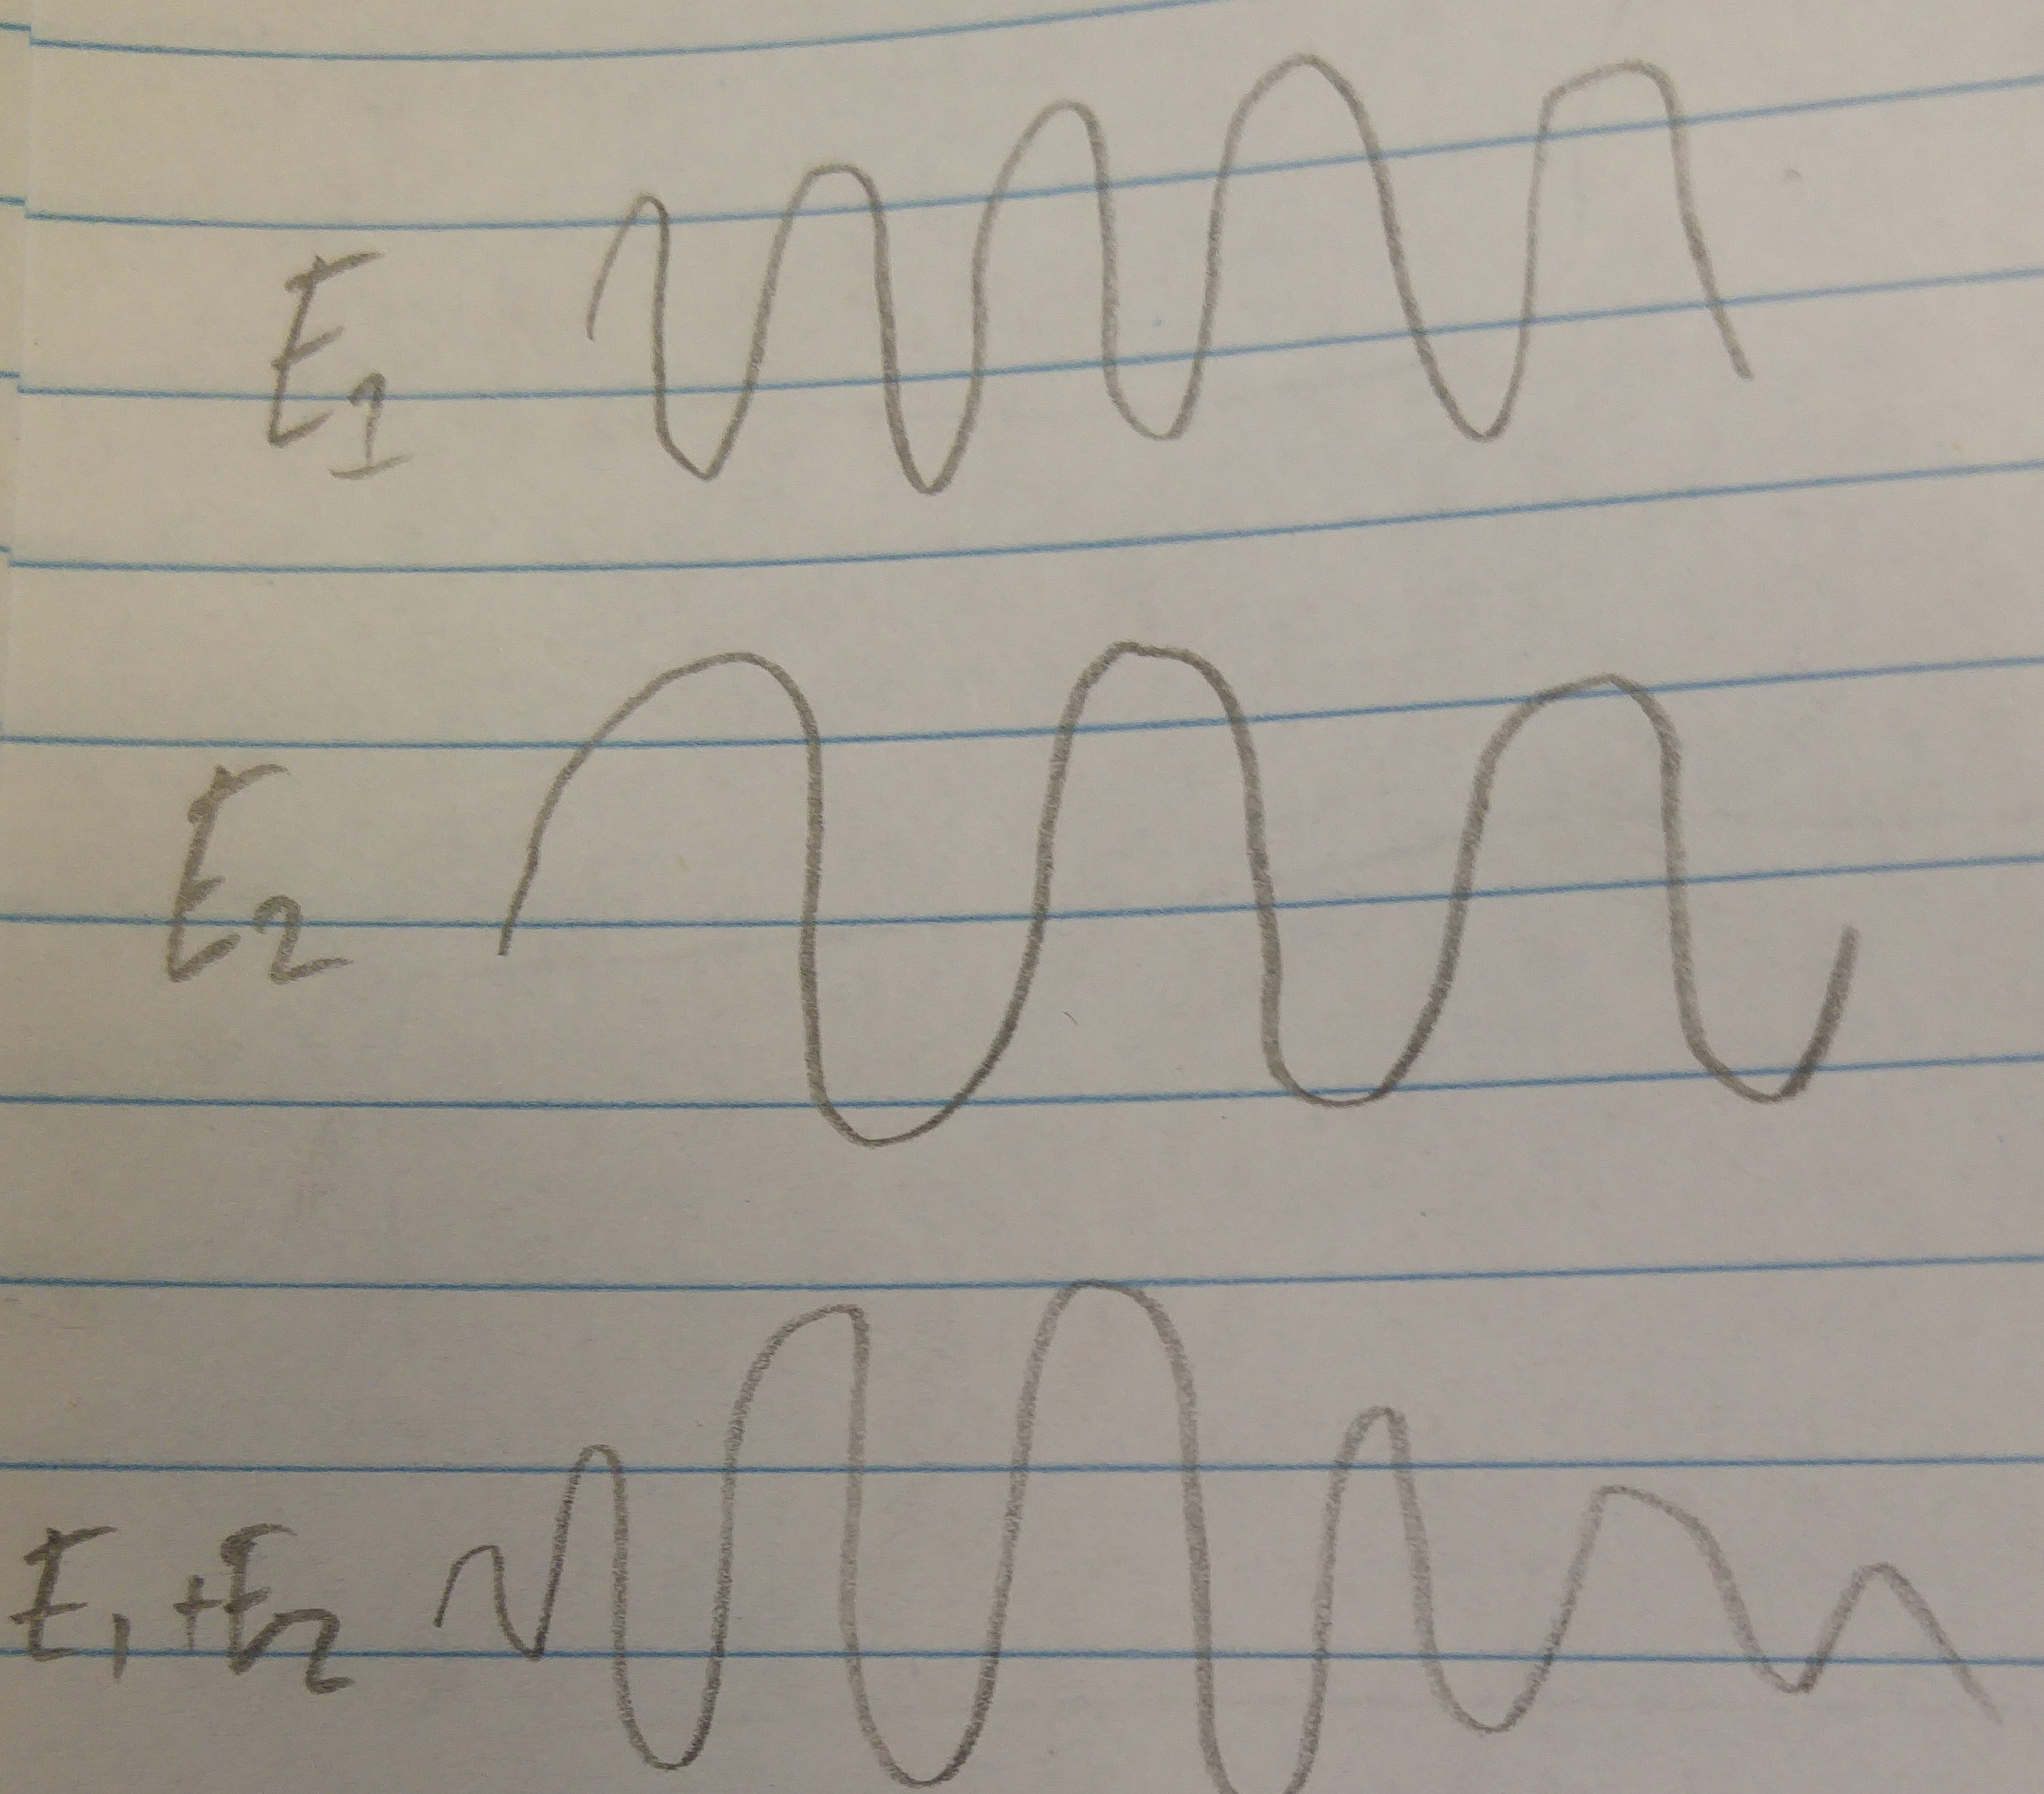
\includegraphics[width=0.5\linewidth]{part1/Figs/beatnote.jpg}
\caption{Depiction of simple beatnote.}
\label{figure:simple_beatnote}
\end{figure}

\subsection{Self-heterodyne}

Self-heterodyne is...

Single delay...

How much delay?

Multipass delay...

These are the results I got...

They look good... too good.

Here's why...\cite{richter_linewidth_1986}

\section{Frequency Reference}
\begin{itemize}
\item Identical laser
\item Narrow laser
\item Three Gaussian lasers
\end{itemize}

\subsection{from paper - merge}
To investigate the discrepancy between the two laser linewidth measurements we used heterodyne measurements which are insensitive to amplitude noise.
Heterodyne measurements were made by frequency shifting one of the laser beams with a double-pass \gls*{aom} and combining the two locked beams on a 50:50 beamsplitter followed by a \unit[1]{GHz} bandwidth photodetector.
The beatnote spectrum was measured with a radio frequency spectrum analyzer, see Fig.~\ref{beatnote}.
Most of the optical power is within the central peak of the spectrum, with \unit[-3]{dB} full width of \unit[$2.0\pm1.1$]{kHz} determined from a Gaussian fit.
The lasers are uncorrelated and if they have identical, Gaussian lineshapes then the single laser \gls*{rms} linewidth is \unit[$0.60\pm0.32$]{kHz}.
The shoulders in the spectrum around \unit[$\pm1.5$]{MHz} correspond to the servo bump of the fully locked spectra in Fig.~\ref{fig:PSDs}.

{\color{red} Rob to determine single laser linewidth from \unit[-3]{dB} beatnote width}

\begin{figure}[htbp]
\centering
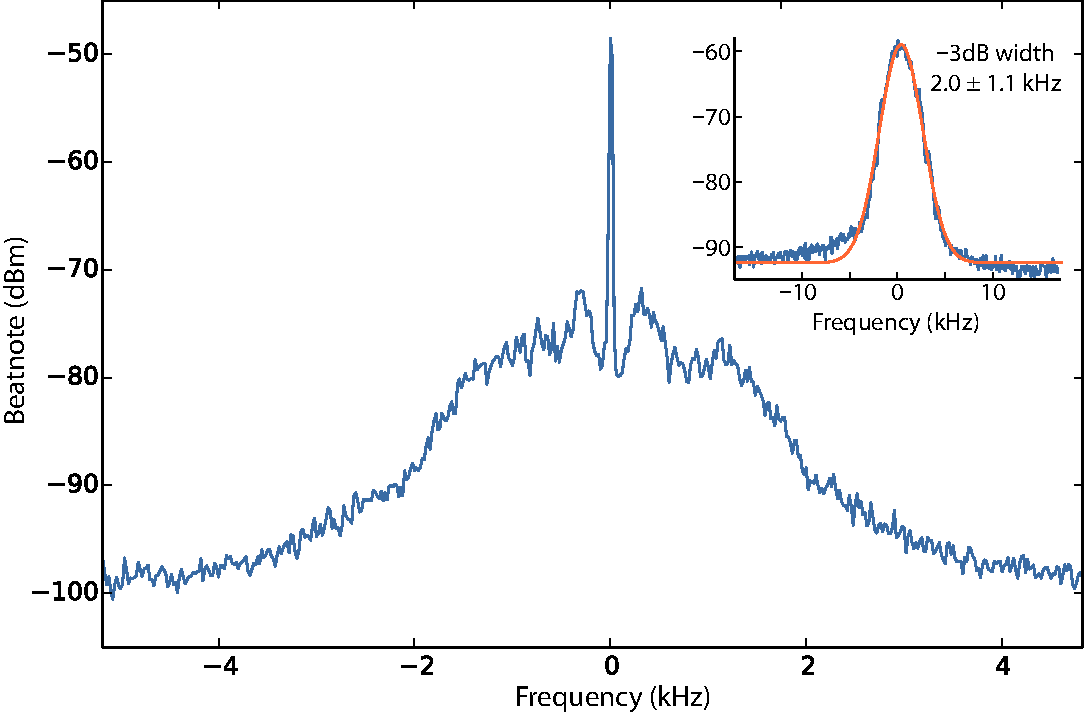
\includegraphics[width=\linewidth]{part1/Figs/fig5_v1.pdf}
\caption{Heterodyne beatnote for the two lasers locked with \gls*{ps}.
The inset figure is a higher resolution measurement of the central peak with a Gaussian fit (red), \unit[-3]{dB} width of \unit[2.0$\pm$1.1]{kHz}.
Both figures are 50 shot averages with resolution bandwidths of \unit[30]{kHz} and \unit[100]{Hz} and total measurement times of approximately \unit[0.5]{s} and \unit[2]{s} respectively.}
\label{beatnote}
\end{figure}

\begin{table}[htbp]
\centering
\begin{tabular}{c c c}
\hline
  & Method & RMS Linewidth (kHz) \\ \hline
  (i) & Cavity transmission mapping  & $2.0 \pm 0.4$ \\
  (ii) &Cavity transmission integral & $2.4 \pm 1.0$ \\
  (iii) & Heterodyne & $0.60\pm0.32$ \\ \hline\end{tabular}
\caption{Linewidth results.
(i) Mapping the transmission signal through a cavity with a \gls*{fwhm} of \unit[71.6]{kHz} to a Lorentzian signal followed by deconvolving from the amplitude noise.
(ii) The results from integrating the power-spectral density of the cavity transmission signal (Fig.~\ref{fig:PSDs}) (iii) The heterodyne beatnote (Fig.~\ref{beatnote}).}
\label{linewidth_table}
\end{table}

\section{Noise measurements}
\subsection{From paper - merge}
\begin{figure}[htbp]
\centering
    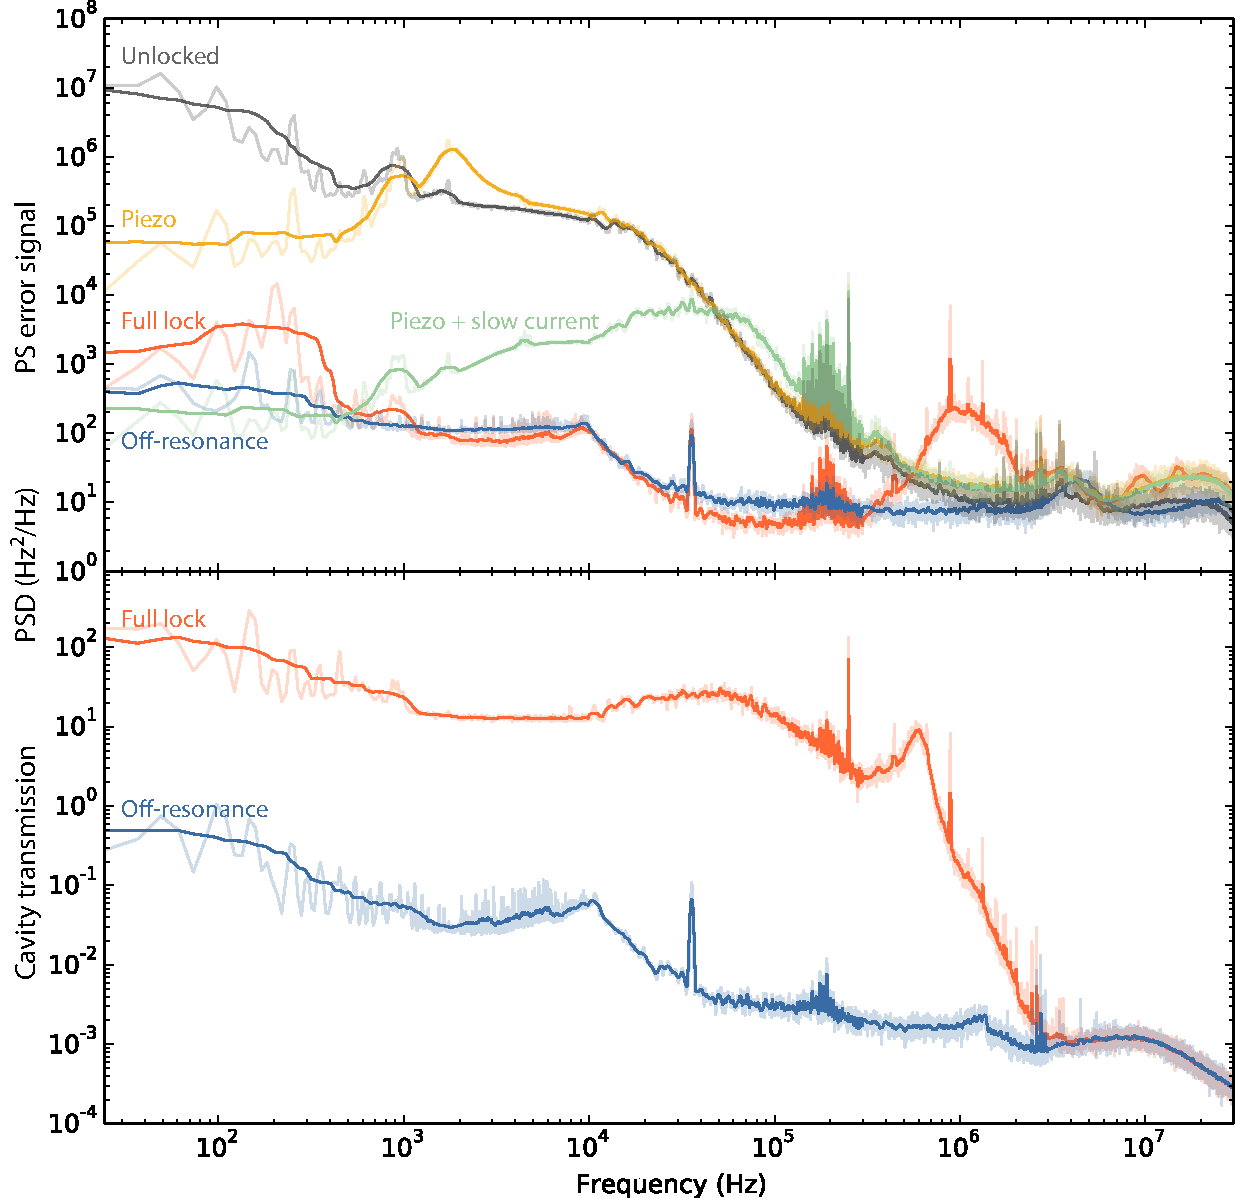
\includegraphics[width=0.9\linewidth]{part1/Figs/fig4a_v3.pdf}
    \label{fig:PSDs}
    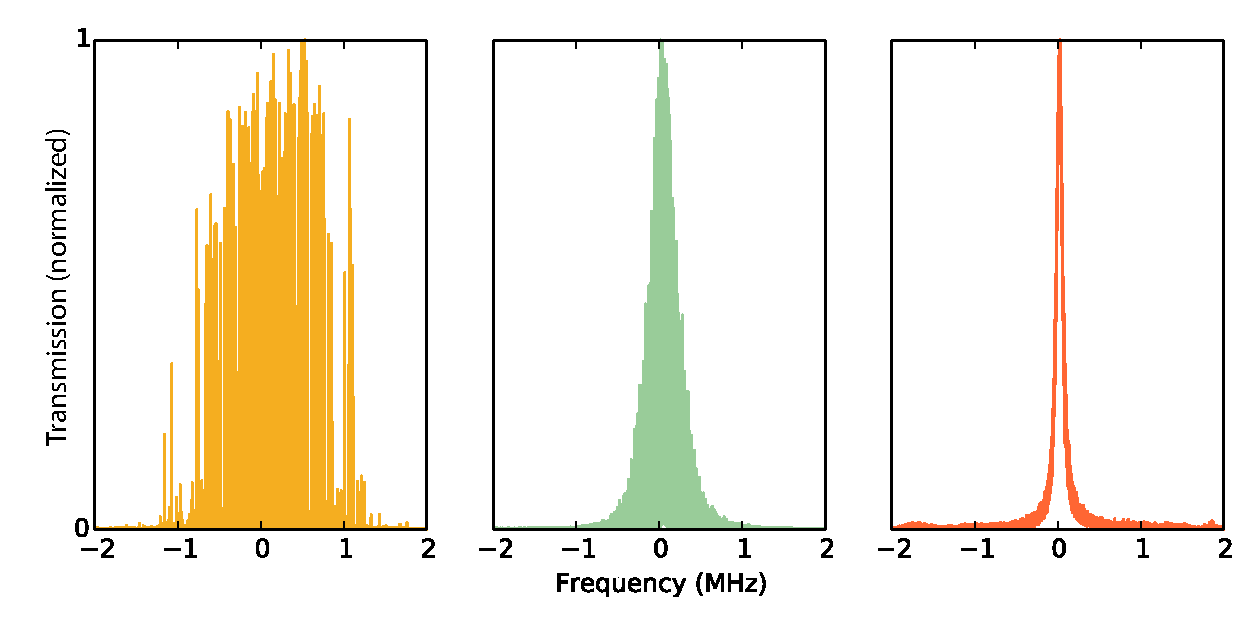
\includegraphics[width=0.9\linewidth]{part1/Figs/fig4b_v1.pdf}
    \label{fig:cavity_scans}
\caption{Frequency noise measurements.
(a) \Gls*{psd} of polarization spectroscopy error signals for a range of laser locking regimes with laser on resonance: unlocked; piezo-only feedback; slow current and piezo feedback; piezo, slow current, and fast AC-coupled current feedback; the noise floor of the noise measurement with no light on the \gls*{ps} detectors.
Laser power \unit[6.5]{mW}.
The measurements are shown with a superposed smoothed curve (moving average  with window size $10\log_{10}(f)$ where $f$ is the frequency).
(b) Optical cavity transmission as a function of laser offset frequency for locking with varying bandwidth.
Piezo only (left), piezo and slow current (middle) and piezo, slow current and fast current (right).
Cavity \gls*{fwhm} linewidth \unit[71.6]{kHz}, scan time \unit[100]{ms}, laser power \unit[170]{$\mu W$}.
(c) \Gls*{psd} of transmitted cavity signal at half peak height for the piezo, slow current and fast AC-coupled current feedback.
For (a) and (c) noise below \unit[$10^4$]{Hz} was measured with a high dynamic range audio digitizer with a resolution bandwidth (RBW) of \unit[12]{Hz}; an RF spectrum analyzer was used at higher frequencies, with RBW of \unit[30]{Hz} between \unit[$10^4$]{Hz}\textendash\unit[$10^6$]{Hz} and RBW of \unit[300]{Hz} above \unit[$10^6$]{Hz}} 
\end{figure}

\subsection{Error Signal Noise}
The spectrum of the \gls*{ps} error signal provides a measure of the laser frequency noise in combination with the \gls*{ps} frequency discrimination, photodetector and electronic noise and gain.
The response of the system to different feedback parameters and the underlying noise limitations are immediately apparent.
The frequency noise \glsfirst*{psd} of the \gls*{ps} error signal (Fig.~\ref{fig:PSDs}) was measured for different feedback configurations, using a high-dynamic-range audio digitizer (low frequency, \unit[\textless10]{kHz}) and radio-frequency spectrum analyzer (high frequency, \unit[10]{kHz} to \unit[30]{MHz}).
The spectrum analyzer was calibrated using the slope of the error signal at resonance.
The low frequency data were calibrated by matching to the spectrum analyzer data at \unit[10]{kHz}.  

Increasing suppression of noise is readily apparent as the feedback bandwidth is increased from \unit[1]{kHz} (piezo only) to \unit[50]{kHz} (piezo and slow current through the laser controller) and then full lock with feedback via direct diode current modulation.
From around \unit[450]{Hz} to \unit[350]{kHz} the fully locked noise spectrum is coincident with the noise floor measured by detuning the laser far from resonance, and intersects with the unlocked spectrum at \unit[700]{kHz}.
A servo bump peaked at \unit[1.3]{MHz} is consistent with a phase lag in laser diode response to current modulation~\cite{wieman_using_1991}.

\subsection{Cavity Transmission Noise}
The error signal spectra provide useful information for optimising the locking system to reduce the laser frequency noise spectrum.
To measure the laser frequency noise spectrum itself we used a high-finesse optical cavity as an independent laser frequency discriminator.
With finesse of 20942 and free spectral range of \unit[1.50]{GHz}, the optical cavity had \gls*{fwhm} linewidth of \unit[71.6]{kHz}.
Fig.~\ref{fig:cavity_scans} shows cavity transmission signals as the laser frequency incident on the cavity was scanned with a double-pass \gls*{aom}.
The resulting traces provide a clear illustration of the effect of increased locking bandwidth: with piezo-only locking the peak appears broad as the laser jitters around the resonant frequency.
With slow current feedback, the transmission peak shape becomes apparent, and finally we see the effect of high-bandwidth feedback with peak width limited by the cavity finesse, indicating a laser linewidth much smaller than the cavity linewidth.

We analyzed the frequency noise of the laser through the cavity transmission signal by choosing a static \gls*{aom} frequency such that the transmitted power through the optical cavity was half the peak power, where the transmission-frequency response is approximately linear. 

The cavity noise spectrum is shown in the lower portion of Fig.~\ref{fig:PSDs} for full bandwidth AC-coupled locking.
The signal was well above the noise floor, measured with laser frequency between transmission peaks, for frequencies up to the \unit[5.5]{MHz} bandwidth of the photodetector.
 This approach could not be used with lower-bandwidth feedback because the laser linewidth was wider than the cavity transmission.
 Note that the cavity transmission noise floor is three to four orders of magnitude lower than that of the \gls*{ps} error signal, in part due to the much lower laser power (microwatts rather than milliwatts) and hence lower shot noise.

We extracted a measure of the linewidth from the cavity data using two methods: first we mapped the amplitude noise of the locked cavity signal to frequency using the cavity transmission frequency response shown in Fig.~\ref{fig:cavity_scans}.
The standard deviation of the distribution of frequencies gave an \gls*{rms} linewidth of \unit[2.4$\pm$0.4]{kHz}.
We also integrated the power spectral density to find an RMS linewidth \cite{negnevitsky_wideband_2013} of \unit[2.4$\pm$1.0]{kHz}.
Linewidth results are summarized in Table \ref{linewidth_table}.

The cavity transmission spectra and linewidth measurements include contributions from both laser frequency and amplitude noise.
An estimate of the amplitude noise contribution to the spectra was obtained by measuring the photodetector power spectrum without the cavity and thus without frequency noise, with the same incident laser power on the photodetector.
Mapping that noise spectrum to frequency produced a contribution of \unit[1.4$\pm$0.3]{kHz} in the cavity transmission mapping linewidth,  and \unit[0.16$\pm$0.07]{kHz} to the PSD integral linewidth.
As expected, the cavity transmission mapping method is more susceptible to laser amplitude noise. 

Assuming the measurements are uncorrelated convolutions of the frequency and amplitude noise contributions, the linewidth determined from cavity transmission mapping consists of the \unit[1.4$\pm$0.3]{kHz} amplitude noise linewidth in combination with a frequency noise linewidth of \unit[2.0$\pm$0.7]{kHz}.
The difference is likely because the mapping method does not properly include contributions from higher Fourier frequencies; that is, the ``pedestal'' of the laser spectrum which can be seen in a heterodyne measurement.

\section{Side of peak (include basic cavity theory here?)}
\section{Integration}
\section{Measuring Slow Frequency Drifts}
\subsection{to merge}

Polarization spectroscopy is inherently a DC technique, susceptible to low frequency drift ($1/f$ noise).
Drift in the laser power output as the laser alignment drifts, variations in fiber coupling efficiency if fibers are used, variations in the atomic vapor density due to changes in temperature, thermal effects on the waveplates and changes to the electronic gains and offsets can all affect the lock point of PS due to the resulting intensity noise combined with the difficulty in perfectly balancing the polarimeter.

The high-finesse cavity was used as a reference to quantify the long-term drift of the PS locked laser over a period of 60 hours (fig.~\ref{fig:drift}).
Drift in the optical cavity frequency was corrected by reference to a laser AC-locked to the rubidium transition using saturated absorption.
The standard deviation of the PS-locked laser frequency measurements was 51\,kHz, approximately half the standard deviation of the measurements in Ref.~\cite{tiwari_laser_2006} and significantly smaller than the 400\,kHz quoted in Ref.~\cite{lee_frequency_2014}.
The frequency change between 10\,s measurements was on average 5\,Hz, with a standard deviation of 210\,Hz.

\begin{figure}[htbp]
\centering
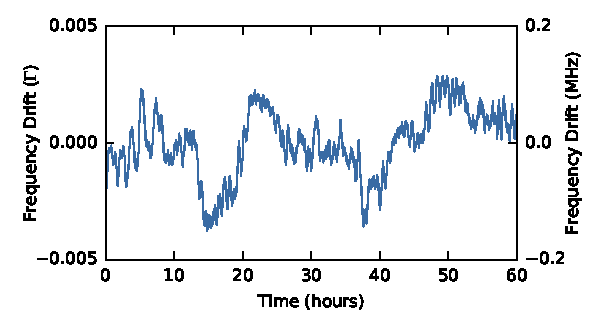
\includegraphics{part1/Figs/drift.pdf}
\caption{Frequency drift of a polarization spectroscopy locked laser, in units of natural linewidth $\Gamma$ and MHz, over a 60 hour period measured every 10 seconds.
The standard deviation of the frequency measurements was 51\,kHz.}
\label{fig:drift}
\end{figure}

The frequency stability of PS is strongly dependent on the extent to which the apparatus is isolated from ambient temperature variations~\cite{yoshikawa_frequency_2003}.
In our system the lasers are temperature stabilized and isolated with acrylic enclosures, and the optical cavity was temperature controlled and isolated inside a vacuum chamber, but the PS and SA components and optical components between lasers and optical cavity were not temperature controlled or shielded from the general laboratory environment.
The locking stability and drift are expected to improve with environmental isolation of all optical components and temperature stabilization of the atomic vapor cell.
The power into the PS setup is particularly sensitive to polarization drift in the light exiting the optical fibers.
Although singlemode polarization maintaining fibers were used, they exhibited significant polarization drift with laboratory temperature variations, and we expect shielded free-space propagation or active power stabilization of the light into the PS setup would further improve the frequency stability.

\section{Bandwidth Stuff}
\subsection{From paper - merge}
\label{bandwidth_section}
The capture range and bandwidth of the frequency discriminator are important in determining the ultimate linewidth that can be achieved, and the ability to compensate for sudden disturbances to the laser frequency, for example due to external shock or vibration.
We define the capture range as twice the minimum frequency difference from resonance for which the locking signal is of the correct sign for negative feedback, which can be deduced from the error signal by locating the first zero crossing to either side of the resonance.
For the spectra shown in Fig.~\ref{sa_ps_spectra} this is greater than \unit[300]{MHz}, many times larger than the \unit[16]{MHz} of \gls*{sa}, as shown in Fig.~\ref{sa_ps_spectra}.

The frequency noise spectrum of the \gls*{ps} error signal is shown in  Fig.~\ref{bandwidth}, both on-resonance and with laser far detuned to determine the noise floor.  The signal and noise intersect at \unit[83]{MHz}.
Since the sign of the \gls*{ps} error signal is constant over that range (see fig.~\ref{sa_ps_spectra}), the \unit[83]{MHz} noise-limited signal bandwidth is indicative of the high bandwidth available from polarization spectroscopy.
In contrast, the \gls*{sa} signal reverses sign several times within \unit[83]{MHz}, and the effective bandwidth is limited by the \unit[$\pm 8$]{MHz} capture range of \gls*{sa}.

\begin{figure}[htbp]
    \centering
    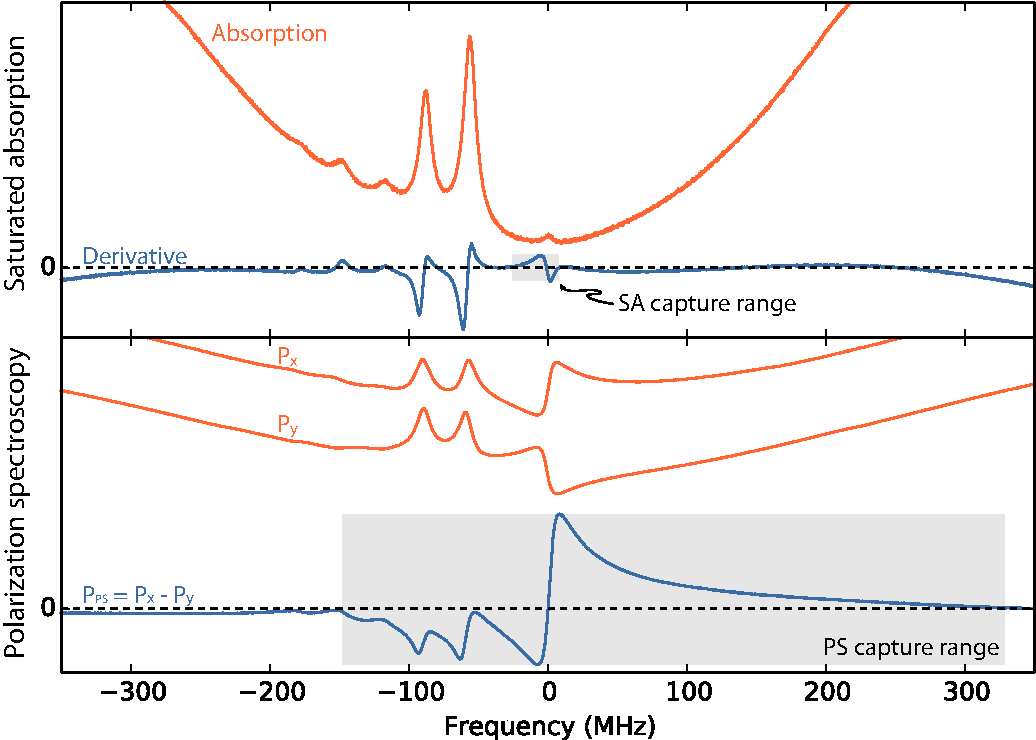
\includegraphics[width=\linewidth]{part1/Figs/fig2_v1.pdf}
    \caption{Saturated absorption spectroscopy (SA) and polarization spectroscopy (PS) spectra for the $^{85}$Rb D2 transition.
The upper portion of the figure shows the absorption and error spectra for SA.
The lower portion shows the components of the PS error signal ($P_{x,y}$ in Fig. \ref{polspec_schematic} and Eq. \ref{P_PS}) and the PS error signal.
The shaded regions indicate the approximate capture range of the respective error signals.
Zero frequency at $^{85}$Rb, $5^2S_{1/2} F=3\rightarrow5^2P_{3/2} F=4$ transition.
Absorption signals normalized to the same maximum absorption on resonance.}
    \label{sa_ps_spectra}
\end{figure}

\begin{figure}[hbp]
    \centering
    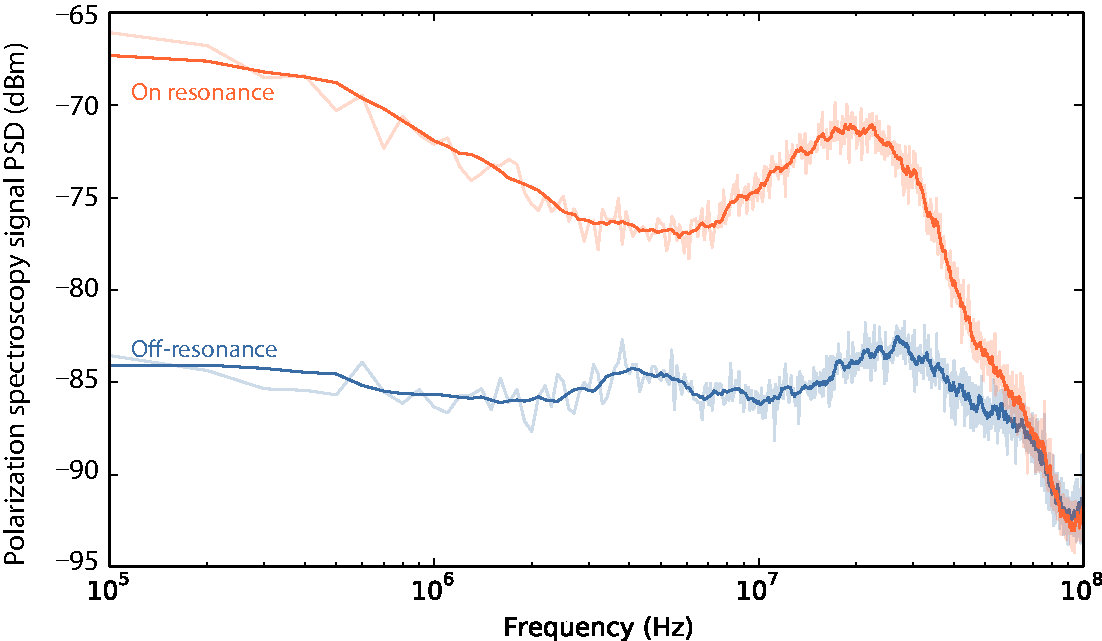
\includegraphics[width=\linewidth]{part1/Figs/fig3_v1.pdf}
    \caption{Polarization spectroscopy error signal frequency noise spectra.
Upper trace (black): frequency spectrum of the error signal while the laser is unlocked and centered on the $^{85}$Rb 5$^\text{2}$S$_\text{1/2}$ $\rightarrow$ 5$^\text{2}$P$_\text{3/2}$ transition.
Lower trace (red): spectrum with laser far from resonance.
The two lines intersect at approximately \unit[83]{MHz}.
Laser power \unit[7.5]{mW} after isolator, with pump:probe ratio 1.4.
The measurements are shown with a superposed smoothed curve (moving 20-point average).}
    \label{bandwidth}
\end{figure}

\section{Long Term Stability}
\subsection{from paper - merge}
Polarization spectroscopy is inherently a DC technique, susceptible to low frequency drift ($1/f$ noise), for example drift in the laser power output as the laser alignment drifts, variations in fiber coupling efficiency, variations in the atomic vapor density due to changes in temperature or local magnetic field, or changes to the electronic gains and offsets.
To quantify the long-term stability, the beatnote between a \gls*{ps}-locked laser and a laser locked to an \gls*{sa} peak was tracked over a number of days.
The \gls*{sa} laser was AC-locked using FM demodulation; that is, with current modulation at \unit[250]{kHz} and demodulation of the detected signal.
FM modulation is inherently insensitive to many of the slow variations that can affect the lock frequency, so that variations in the beatnote frequency can be attributed to the drift in the \gls*{ps} laser.
A linear fit to the beatnote data (Fig.~\ref{drift}) sets an upper limit on the frequency drift of less than \unitfrac[2]{kHz}{h}. 

Others have measured drifts of \unitfrac[17]{kHz}{h} to \unitfrac[1]{MHz}{h}~\cite{yoshikawa_frequency_2003, tiwari_laser_2006} and standard deviation of \unit[400]{kHz} \cite{lee_frequency_2014}, depending on the extent to which the apparatus was isolated from ambient temperature variation.
In our system the lasers are temperature stabilized and isolated from the environment with acrylic boxes, but the \gls*{ps} and \gls*{sa} components were not temperature controlled or shielded from the general laboratory environment.
Polarization and power stabilization of the laser, and temperature stabilization of the atomic vapor cell, are likely to improve the locking stability and drift.

\begin{figure}[htbp]
\centering
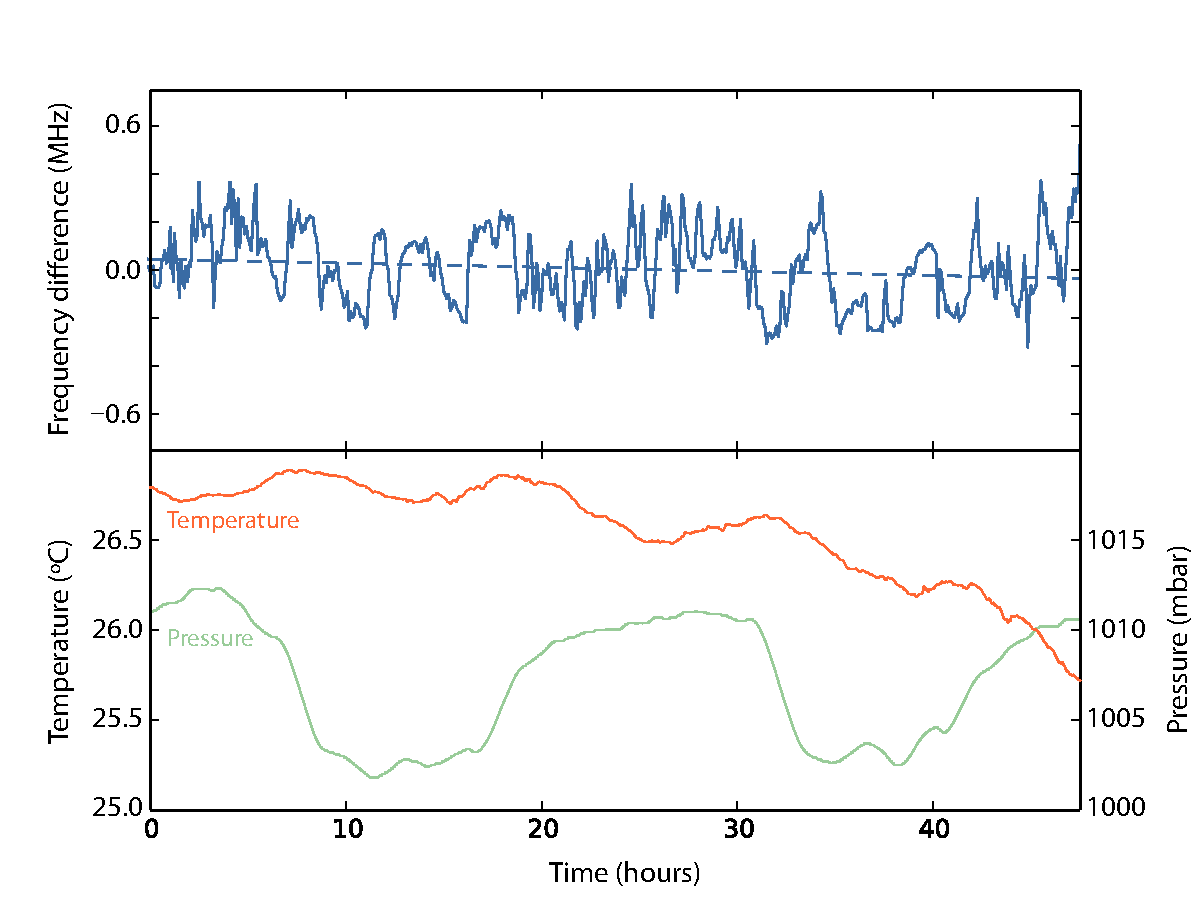
\includegraphics[width=\linewidth]{part1/Figs/fig6_v1.pdf}
\caption{Measurement of frequency drift of a polarization spectroscopy locked laser over a 50 hour period.
Upper: frequency deviation and linear fit with gradient \unitfrac[-1.7]{kHz}{h} sets an upper limit to the drift.
The standard deviation of the frequency measurements, acquired at \unit[5]{min} intervals, was \unit[155]{kHz}.
Lower: temperature (dotted line) and pressure (dashed line) of the laboratory over the same period of time, measured every \unit[200]{ms}.}
\label{drift}
\end{figure}

\section{Conclusion}
We have demonstrated laser frequency stabilization using a polarization spectroscopy reference, and reduced the linewidth of \gls*{ecdl} lasers well below \unit[1]{kHz}, much lower than previously demonstrated with this technique and previously achieved only by locking to high-finesse optical cavities.
The absolute frequency drift of less than \unit[50]{kHz} per day is adequate for many laser cooling experiments.
Further improvements to drift could be achieved with simple measures such as temperature stabilization and environmental isolation.
The experimental setup provides an approach with low complexity and low cost, providing wide bandwidth linewidth narrowing without radio frequency modulation while retaining an absolute atomic reference.

In our experiments, the locking bandwidth is limited by the phase lag in the laser diode response to injection current variation, to around \unit[700]{kHz}.
With appropriate servo loop shaping, for example multiple phase lead stages to compensate for the diode response, it is reasonable to expect a bandwidth increase to several MHz.
However, the effect on linewidth would be negligible because the \gls*{ps} signal-to-noise ratio is small in this frequency range.
Much greater improvements could be made by lowering the \gls*{ps} noise floor, which is three to four orders of magnitude higher than the noise floor of the optical cavity.
The difference is only partly due to the $100\times$ higher power in \gls*{ps}, which will increase shot and Johnson noise by $10\times$.
 More...
